% Copyright 2023 The terCAD team. All rights reserved.
% Use of this content is governed by a CC BY-NC-ND 4.0 license that can be found in the LICENSE file.

\newpage
\subsection{Assessing of Ignorance} \label{ut-fail}
\markboth{Gating}{Assessing of Ignorance}

Initially, we emphasized the importance of having tests and an ecosystem for their automation. However, we did not write 
anything about the repercussions of neglecting them. Now, let's review the errors made during our increment (four 
iterations, two weeks each).

\begin{lstlisting}[language=terminal]
git log --format="%ad %s" --grep="\[BF\]" --date=iso | awk -F ' ' '{print $1}' | sort | uniq -c
\end{lstlisting}

\noindent \q{git log}-command retrieves a commit history (\q{\%ad} - to include the commit date, \q{--date=iso}-option 
converts dates to ISO 8601 [YYYY-mm-dd]; \q{\%s} - take subject) with the specified format via \q{--grep} (since we've 
used \q{[BF]}-prefix in a title for created bug-reports [issues] and used it as a part of the commit message). \q{awk} 
extracts the date part from each line and delegate sorting to \q{sort}-command by the extracted dates. Finally, 
\q{uniq -c}-command counts the occurrences of each unique date. And the same operation we'll do for the \q{fix}-keyword.

\begin{figure}[h]
  \begin{center}
    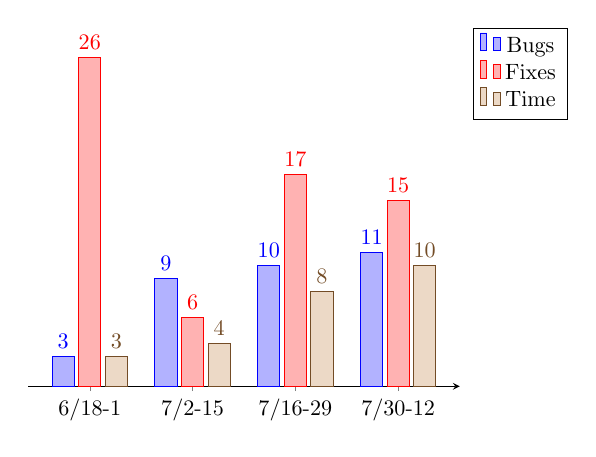
\begin{tikzpicture}[scale=0.8]
      \begin{axis}[ybar, symbolic x coords={6/18-1, 7/2-15, 7/16-29, 7/30-12},
        legend pos=outer north east, axis y line=none, axis x line=bottom, nodes near coords, enlarge x limits=0.2, ] 
      \addplot+ coordinates {(6/18-1, 3) (7/2-15, 9) (7/16-29, 10) (7/30-12, 11)}; 
      \addplot+ coordinates {(6/18-1, 26) (7/2-15, 6) (7/16-29, 17) (7/30-12, 15)}; 
      \addplot+ coordinates {(6/18-1, 3) (7/2-15, 4) (7/16-29, 8) (7/30-12, 10)}; 
      \legend{Bugs, Fixes, Time}; \end{axis} 
    \end{tikzpicture} 
  \end{center}
  \caption{Counting made mistakes per each Iteration}\label{graph:errors}
\end{figure}

\noindent In the resulting \cref{graph:errors}, the data is presented as follows:
\q{Time} -- indicates the number of hours that were allocated to resolving identified issues during an Iteration (as a 
note, the total allocated time per iteration was 28 hours);
\q{Bug} -- represents the number of identified bugs within the project;
\q{Fixes} -- corresponds to the number of mentioned fixes made from our Git history.

Current project was spearheaded by a lone developer, while additional team members could potentially increase 
the needed efforts \cite{Alm21} to maintain the application stability. Returning back to our chart, it shows us 
that up to a third of the allotted time was spent on fixing bugs -- by adhering to the principle of zero 
defects distribution \cite{Allan98}. In the business realm, companies sometimes opt to overlook issues and instabilities 
while augmenting functional capabilities through the introduction of new features. This can inadvertently create a ticking 
time bomb, culminating in substantial financial and reputational losses. That's why the cost to brand perception is 
frequently greater than the cost of finding and fixing a bug during development. By example, National Institute of 
Standards and Technology found that software bugs cost (in 2002) the US economy \$59.5 billion every year, and 
\$22.2 billion could be eliminated by improved testing \cite{RTI02}.

Simply saying, the consequence of missed tests is a broken managerial triangle: out from a scope, time, and budget.
Neither Agile transformation, nor micromanagement would help to be predictive in delivery. To mitigate potential adverse 
outcomes, a widely adopted strategy involves instigating a technical iteration, or designating a specific period, often 
at the close of a calendar year, for dedicated bug-related work. As a testament to robust processes, the fundamental 
principle of quality permeates all stages and serves as a cultural cornerstone. Non-functional requirements, serving 
as a tool to ensure quality throughout every phase, can find a practical application here \cite{Sam17}, \cite{Suz12}. 
The strength of a system is determined by the resilience of its most vulnerable component. That's why we should always 
bet on tests automation, it won't be regretted.

The Test-Driven Development approach has been around since 1999 as the Extreme Programming flow, but for unknown 
reasons, it has not become widely popular. The argument that "we don't have time to write tests" is similar to saying, 
"We won't use a car to reach our 200 km target since we can already run that distance within a day". In 
Agile transformations, the mantra is that using Scrum, a communication framework, will increase development flow 
tenfold. More broadly, Agile, DevOps, Lean, and other approaches emphasize quality throughout the process. This is 
because communication itself has a natural limitation on achievable performance optimization. The next 10x boost can be 
achieved by growing technical excellence exceptionally. When we observe developers dedicating half a day to testing a 
seemingly "one-hour" change, it's perplexing that the idea of investing an additional hour in crafting tests is met with 
resistance.

For example, achieving technical excellence through a semaphore approach ("red" — write a test for the missing part of 
the code and assert expectations; "yellow" — write code to pass the tests; "green" — refactor the code) eliminates the 
need for a stabilization phase, monthly regression testing, and a separate QA department. All acceptance criteria for a 
user story, feature, or epic are translated into tests and controlled by automation. This approach reinforces the 
developer's mental model of the code, boosts confidence, and increases productivity.
